\documentclass[svgnames,smaller,table]{beamer}
\usepackage{multirow}
\usepackage{tikz}
\usefonttheme[onlymath]{serif}

\usepackage{listings}
% Configura o listings
\lstset{
  %  basicstyle=\footnotesize,\small,...\tiny
  basicstyle=\ttfamily\scriptsize,
  commentstyle=\color{mygreen},
  numbers=left,
  stepnumber=1,
  showstringspaces=false,
  tabsize=2,
  breaklines=true,
  breakatwhitespace=false
 columns=fixed,
 fontadjust=true,
 basewidth=0.5em
}


\usetheme{lthn}
\setbeamercolor*{normal text}{fg=black}
% -----------------------------------------------------------------------------------------------------------------

\title[Transparência]{Cluster LTHN: Visão Geral e Utilização básica}
\author{Vitor Vasconcelos Araújo Silva}
\date{\today}
\institute{%
  LTHN - Laboratório de Termo-hidráulica e Neutrônica
  \par
  Serviço de Tecnologia de Reatores - CDTN}

\begin{document}

%-------------------------------------------------
\begin{frame}
\titlepage
\end{frame}

%-------------------------------------------------
\begin{frame}
  \frametitle{Sumário}
  \tableofcontents[pausesections]
\end{frame}


\section{O cluster}
%-------------------------------------------------
\begin{frame}
  \frametitle{O cluster}
  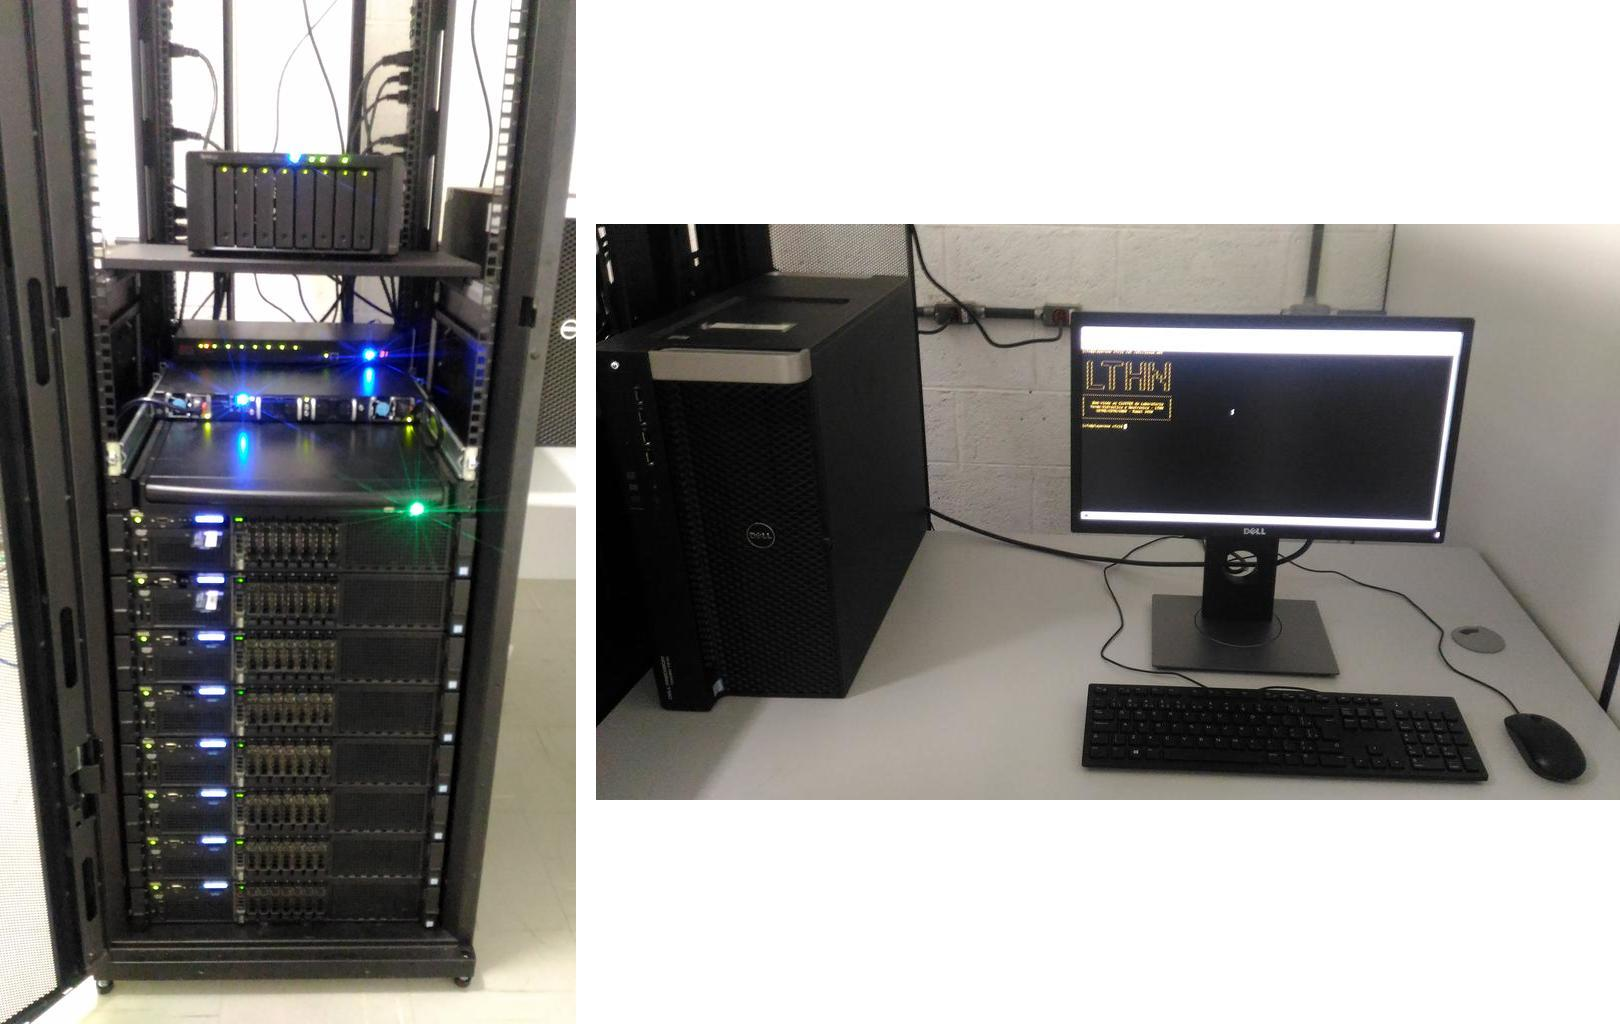
\includegraphics[scale=0.2]{figuras/duas.jpg}
\end{frame}

\subsection{Visão Esquemática}
%-------------------------------------------------
\begin{frame}
  \frametitle{O cluster}
  \framesubtitle{Visão esquemática}
  \begin{center}
    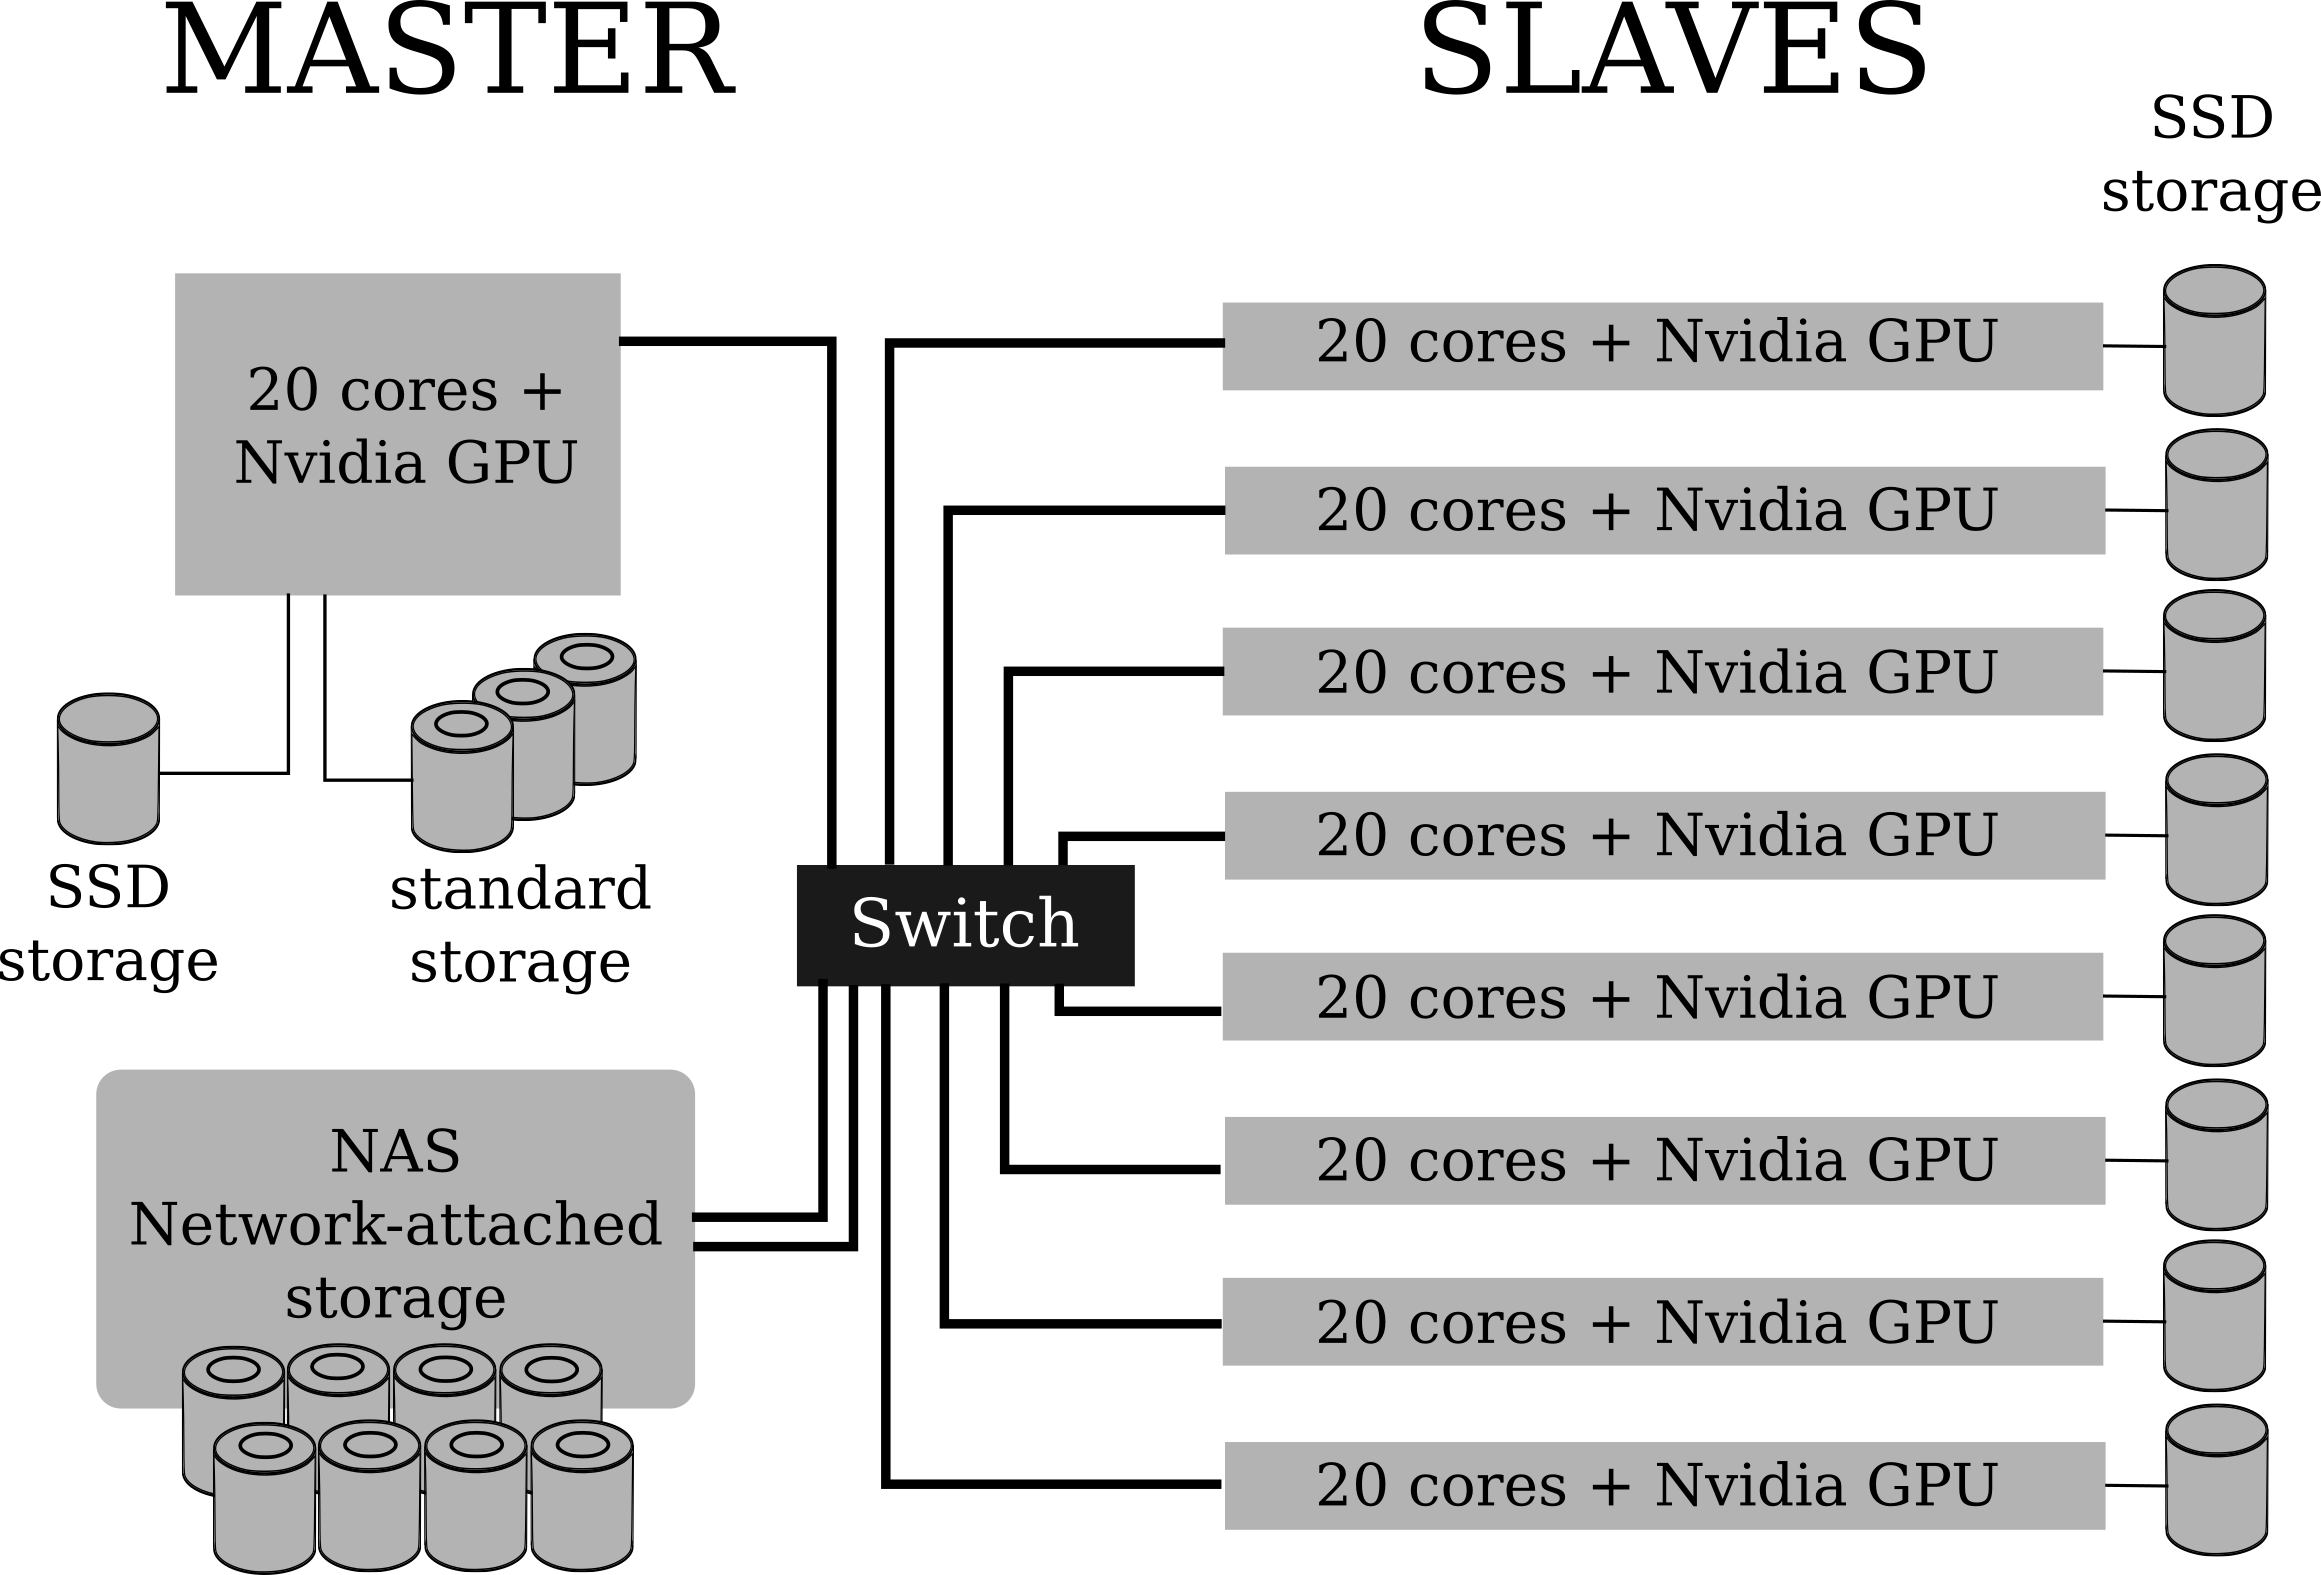
\includegraphics[scale=0.5]{figuras/cluster-topologico.png}
  \end{center}
%  \begin{tikzpicture}[remember picture,overlay]
%    \node[anchor=center, inner sep=0] (img1) at (0,0) {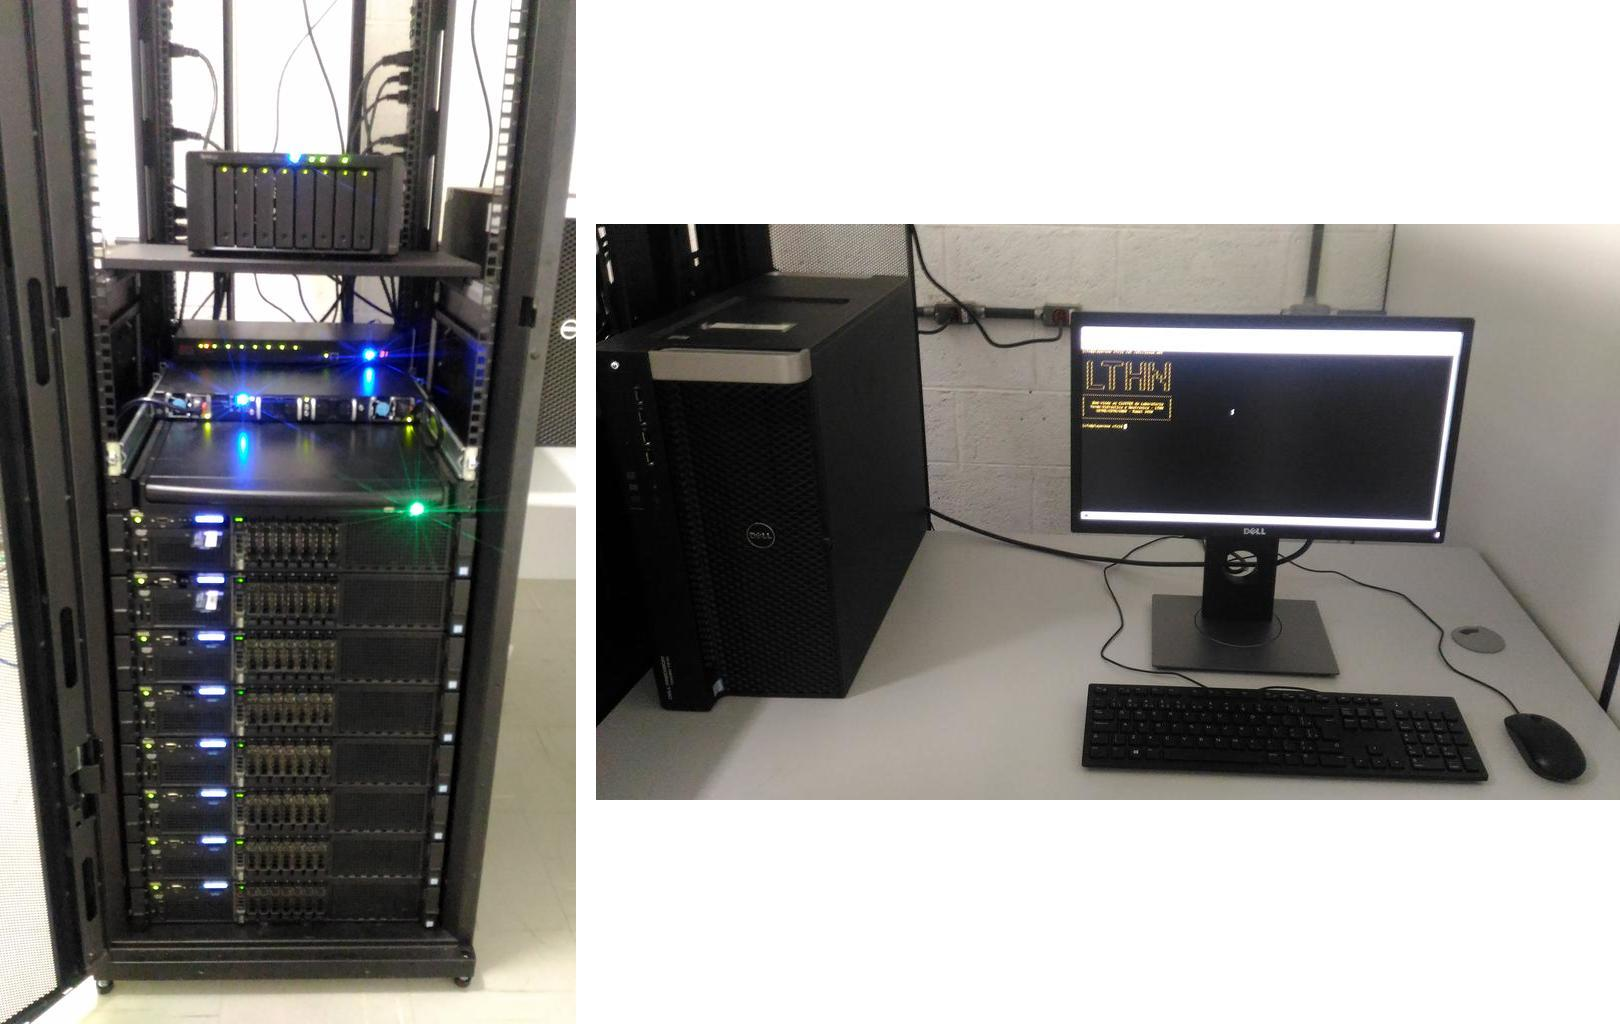
\includegraphics[scale=0.2]{figuras/duas.jpg}};
%    \begin{scope}[
%        x={(img1.south east)},
%        y={(img1.north west)}
%      ]
%      \node [red, font=\bfseries] at (0.25,0.65) {$P(X|Y)$};
%    \end{scope}
%  \end{tikzpicture}
\end{frame}

%-------------------------------------------------
\begin{frame}
  \frametitle{Gluster: o que é?}
  \framesubtitle{Sistema de arquivos distribuído \textbf{GlusterFS}}

\textbullet  \textit{Free and open source software}:\\% exatamente! Gratuito e de código aberto (não que pensemos em modificá-lo...)\\
\textbullet  Nativo para \textit{CentOS}: instalação e atualizações fornecidas via repositório e compatibilidade garantida.\\
\textbullet  Modelo cliente servidor;\\
  \vspace{0.2cm}
  (Algumas) Funcionalidades:

  \begin{enumerate}
  \item Espelhamento
  \item Replicação
  \item \textit{Striping}
  \item Tolerância a falhas
  \item Cotas
  \end{enumerate}

\end{frame}


%-------------------------------------------------
\begin{frame}
  \frametitle{Gluster: o que é?}
  \framesubtitle{Sistema de arquivos distribuído}
    \begin{center}
      \includegraphics[scale=0.65]{figuras/gluster.png}
    \end{center}
\end{frame}

%-------------------------------------------------
\begin{frame}[fragile]
  \frametitle{Gluster: o que é?}
  \framesubtitle{Volumes na prática}
  \begin{lstlisting}
    gluster volume info
    fdsafdsa
    fdsafdsa
    fdsafdsa
  \end{lstlisting}
\end{frame}

%-------------------------------------------------
\begin{frame}
  \frametitle{O cluster}
  \framesubtitle{Na prática, um grande ``disco'' de armazenamento}
    \begin{center}
      \includegraphics[scale=0.45]{figuras/cluster-gluster.png}
        \end{center}
\end{frame}

%-------------------------------------------------
\begin{frame}
  \frametitle{O cluster}
  \framesubtitle{Na rede do CDTN}
  \begin{center}
    \includegraphics[scale=0.45]{figuras/cluster-rede.png}
  \end{center}
  
%  \begin{tikzpicture}[remember picture,overlay]
%    \node[anchor=center, inner sep=0] (img1) at (0,0) {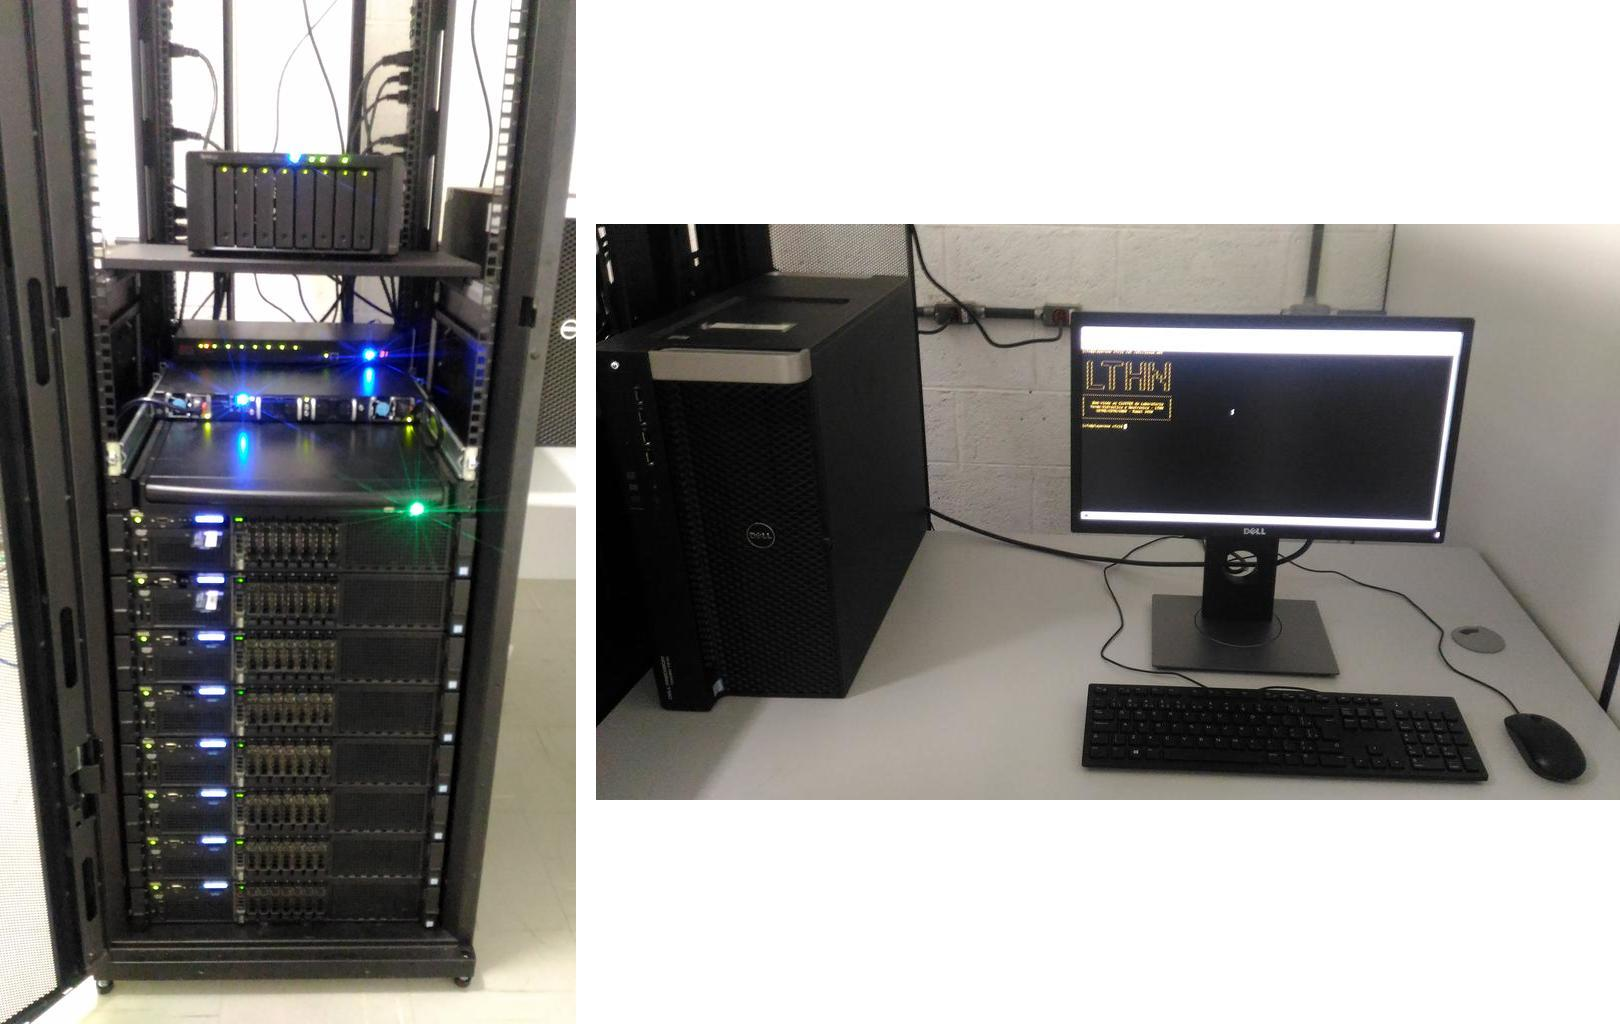
\includegraphics[scale=0.2]{figuras/duas.jpg}};
%    \begin{scope}[
%        x={(img1.south east)},
%        y={(img1.north west)}
%      ]
%      \node [red, font=\bfseries] at (0.25,0.65) {$P(X|Y)$};
%    \end{scope}
%  \end{tikzpicture}
\end{frame}


\subsection{Características}
%-------------------------------------------------
\begin{frame}
  \frametitle{O Cluster}
  \framesubtitle{Hardware}
  1 mestre bla bla bla\\
  8 máquinas bla bla bla.
  \\
  \vspace{0.5cm}
  32 Gb RAM cada.
  (256Gb RAM para o mestre)
  \vspace{0.5cm}
  Nada
  \begin{itemize}
  \item Apesar disso, útil e aplicável em situações práticas
  \item Resolvida por métodos numéricos utilizando \textbf{discretização de domínio};
  \end{itemize}
\end{frame}

%-------------------------------------------------
%{\setbeamercolor{background canvas}{bg=black}
%  \setbeamercolor{frametitle}{fg=red}
%  \setbeamercolor{normal text}{fg=red}
%  \usebeamercolor[fg]{normal text}

\subsection{Software}
\begin{frame}
  \frametitle{Software}
  \framesubtitle{O que temos disponível?}
%\centering
\begin{itemize}
	\item \textbf{Serpent2 Monte Carlo};
	\item \textbf{MCNP 6};
	\item \textbf{OpenFOAM versão 6};
	\item \textbf{Pacote ANSYS};
	\item \textbf{SCALE 6.2.3};
	\item \textbf{Matlab}.
\end{itemize}

\end{frame}
%}

\subsection{Ganglia}
%-------------------------------------------------
\begin{frame}
  \frametitle{Sistema de Monitoramento}
\end{frame}



%-------------------------------------------------
\begin{frame}[fragile]
  \frametitle{Acesso à memória compartilhada - Criação}
%  \framesubtitle{Exemplo1}
 \begin{lstlisting}%[caption={Fragmento do código-fonte da criação das estruturas de memória compartilhada.}\label{lst:createshm}]
   // Three C standard arrays are created to shared data with milonga
   double *shmTarray = NULL;
   double *shmQarray = NULL;
   
   void *shmT;
   void *shmQ;

   int shmTfile = 0;
   int shmQfile = 0;
   
   // Posix C semaphores
   sem_t *calcOf;
   sem_t *calcMil;
   
   // Posix structures initialization
   calcOf = sem_open("calcOf", O_CREAT, 0666);
   calcMil = sem_open("calcMil", O_CREAT, 0666);
   
   if(Pstream::master())
   {
     // Semaphores and shared memory files are tested at this point.
     // If milonga is not running, OpenFOAM runs uncoupled.
     shmTfile = shm_open("temperaturas", O_RDWR, 0666);
     shmQfile = shm_open("potencias", O_RDWR, 0666);
    
     if(shmTfile == -1 || shmQfile == -1) coupling = false; // Error finding shared memory
   }
 \end{lstlisting}
\end{frame}


\section{Utilização prática}
%-------------------------------------------------
\subsection{SLURM}
\begin{frame}
  \frametitle{\textit{Slurm Workload Manager}}
%  \framesubtitle{}
  \textbullet Sistema de controle de tarefas (\textit{jobs}).\\
  \vspace{0.2cm}
  \textbullet \alert{\textbf{Única}} forma de utilizar os recursos\footnote[frame]{Tecnicamente esta afirmativa não é verdadeira}.\\
  \vspace{0.2cm}
  \begin{itemize}
    \item \texttt{sinfo}
    \item \texttt{squeue}
    \item \texttt{srun}
    \item \texttt{sbatch}
    \item texttt{cancel}
  \end{itemize}
%  \centering
%  \vspace{0.2cm}
%  \begin{tabular}{lrrrr}
%    \multicolumn{5}{c}{Temperaturas dos materiais}                                                                                                       \\ \hline
%    & \multicolumn{1}{l}{$T_1${[}K{]}} & \multicolumn{1}{l}{$T_2${[}K{]}} & \multicolumn{1}{l}{$T_3${[}K{]}} & \multicolumn{1}{l}{$T_4${[}K{]}}      \\ \hline
%    Combustível  & 300                             & 400                             & 500                             & 600                             \\ \hline
%    Revestimento & 300                             & 396                             & 403                             & 410                             \\ \hline
%    Refrigerante & 300                             & 308,5                           & 317                             & 341                            
%  \end{tabular}
\end{frame}

%-------------------------------------------------
\begin{frame}
 \vfill
  \begin{beamercolorbox}[center]{title}
     \Huge{Muito obrigado!}
  \end{beamercolorbox}
  \vfill

\end{frame}

%-------------------------------------------------
\begin{frame}[allowframebreaks]
        \frametitle{Referências}
        \bibliographystyle{amsalpha}
        \bibliography{apre.bib}
\end{frame}


%-------------------------------------------------
% Frame escondido
\begin{frame}[noframenumbering]
  \frametitle{Respostas}
  \framesubtitle{Seções de choque}
  Tratamento complexo.
\end{frame}


\end{document}

